\documentclass[a4,12pt]{article}
\usepackage[T1]{fontenc}
\usepackage{textcomp}
\usepackage[utf8]{inputenc}
\usepackage[english]{babel}
\usepackage{graphics}
\usepackage{graphicx}
\usepackage{epstopdf}
\usepackage{amsmath}
\usepackage{hyperref}
\usepackage{fancyvrb}
\usepackage{verbatim}
\usepackage{cmap}
%\renewcommand{\familydefault}{\sfdefault}
\textwidth=16cm
\oddsidemargin=0.1cm
\linespread{1.2}

\newcommand{\HRule}{\rule{\linewidth}{0.5mm}}
\DefineVerbatimEnvironment{code}{Verbatim}{frame=single, fontsize=\small}

\begin{document}

\begin{titlepage}

\begin{center}

% Title
\HRule \\[0.4cm]
{ \huge \bfseries Portable accelerated kernels generator\linebreak for Fortran programs}\\[0.4cm]

\HRule \\[0.5cm]

\textsc{\Large report}\\[1.5cm]


\vfill

% Bottom of the page
{\large \today}

\end{center}

\end{titlepage}

\begin{abstract}

FF

\end{abstract}

\section{Section}

FF

\begin{figure}
\centering
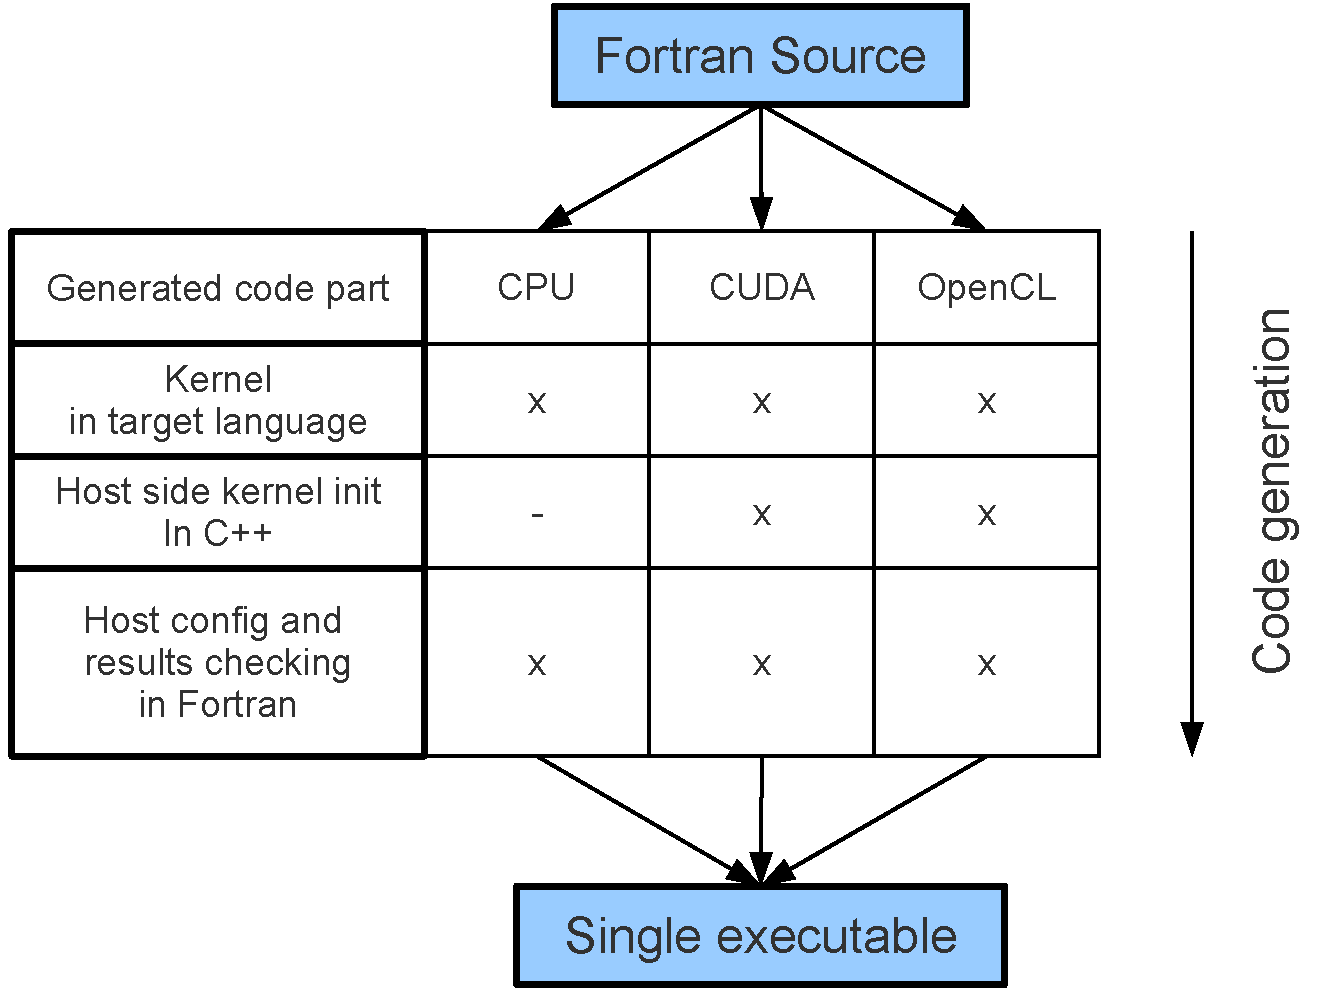
\includegraphics[scale=0.5]{figures/portability.pdf}
\caption{Portability}
\label{fig:portability}
\end{figure}

\begin{figure}
\centering
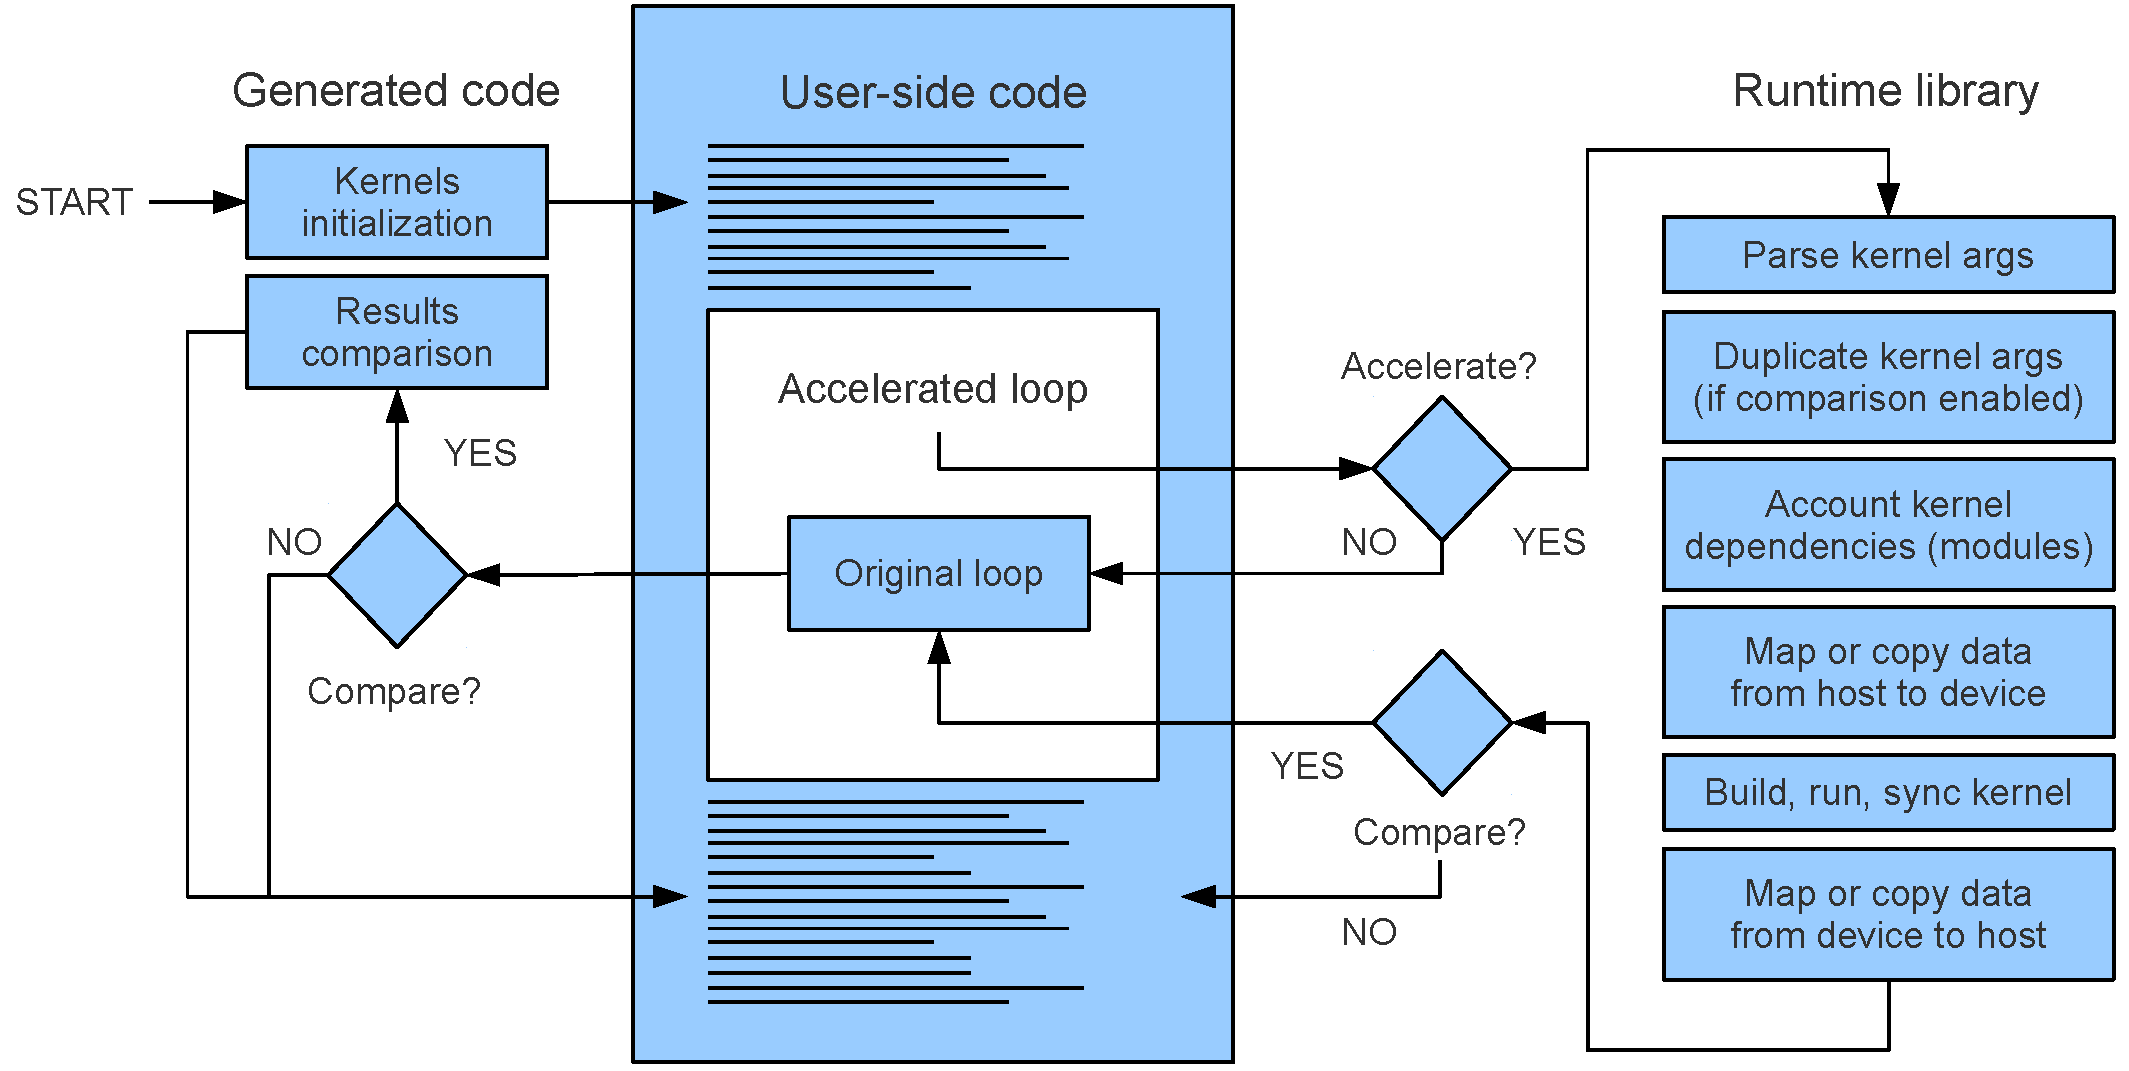
\includegraphics[scale=0.4]{figures/execution.pdf}
\caption{Execution model}
\label{fig:execution}
\end{figure}

\end{document}
